\chapter{Abordagem da Engenharia de Requisitos}

  Scaled Agile Framework, ou SAFe, é utilizado para dimensionar processos ágeis para grandes projetos. Uma das filosofias do processo
  ágil é uma equipe pequena auto gerenciavel, porém, por meio do SAFe, é possível garantir esse nível de auto gerenciamento em uma
  grande quantidade de equipes trabalhando em um mesmo projeto.

  Como o SAFe é baseado em processos ágeis, o framework também compartilha os princípios ágeis. Como por exemplo, o uso do kanban para
  os diferentes níveis, e até mesmo a utilização do scrum no nível mais baixo.

  Além de compartilhar essas características com os processos ágeis, o SAFe possui 9 príncipos, são eles:

  \begin{enumerate}
    \item Ter uma visão econ\^{o}mica
    \item Aplicar um pensamento sistêmico
    \item Assumir variabilidade; preservar opções
    \item Construir incrementalmente de forma rapida, com ciclos integrados de aprendizagem
    \item Se baseie em marcos com o objetivo de avaliação de sistemas funcionais
    \item Visualize e limite trabalhos em andamento, reduzir a quantidade de trabalhos e gerenciar grandes filas de espera.
    \item Utilizar uma cadencia e sincronizar planejamento entre domínios
    \item Habilitar a motivação intrínseca de conhecimento dos trabalhadores
    \item Descentralizar a tomada de decisão
  \end{enumerate}

  O SAFe é divido em 3 níveis: \textbf{portfólio, programa e time.}

\subsection{Portfólio}

  De acordo com o site do framework, o nível de portfólio é voltado para as pessoas e processos que são necessárias para a construção
  de sistemas e soluções que a empresa necessita para atingir uma meta prevista.

\subsection{Programa}

  O nível de programa é onde os times de desenvolvimento e outros recursos são aplicados em alguma solução em desenvolvimento corrente.

\subsection{Time}

  Por fim, o nível de time mesmo que definido como níveis diferentes, é uma parte do nível de programa. Cada time é responsável por
  definir, construir e testar as histórias de seu backlog de time dentro de sprints, e cada um é organizado de acordo com as capacidades
  e talentos de cada indivíduo.

\subsection{Big picture}

  \begin{figure}[!htpb]
	  \centering
	  \includegraphics[scale=0.7]{figuras/abordagem/SAFe_Big_Picture_4}
	  \caption{Big picture do SAFe}
  \end{figure}

\section{Tradicional $-$ RUP}

  A metodologia tradicional nasceu com o crescimento da computação, onde o nascimento de sistemas empresariais e corporativos necessitou
  ferramentas para gerenciar grandes projetos. Uma das metodologias tradicionais mais utilizada é o RUP

  RUP é um framework de processo de engenharia de software que fornece um conjunto de práticas testadas na indústria para desenvolvimento
  de software e gerência de projetos (Shuja, 2007). Como participante da categoria de metodologia tradicional, o RUP é caracterizado em
  fases e/ou etapas, e tem um foco alto na documentação do processo.

  Ele é uma metodologia iterativa, na qual basicamente é constituída em quatro fases e diversas iterações entre elas, na qual tem como
  finalidade tratar questões como planejamento, levantamento e análise de requisitos e entre outros. São elas:

  \begin{itemize}
    \item \textbf{Iniciação}: Tarefas de comunicação com o cliente e o planejamento;
    \item \textbf{Elaboração}: Analisar de forma mais detalhada o domínio do problema;
    \item \textbf{Construção}: Construção e desenvolvimento do software;
    \item \textbf{Transição}: Entrega do software e testes.
  \end{itemize}

  No RUP também tem as disciplinas, que são basicamente atividades distribuídas ao longo das quatro fases, onde descrevem o que deve ser
  feito em cada fase com relação à documentação, atividades e outros.

  \begin{figure}[!htpb]
    \centering
    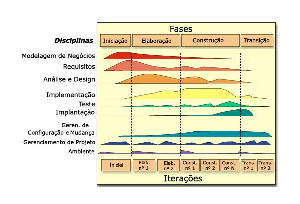
\includegraphics[scale=2.0]{figuras/abordagem/Fases_RUP}
    \caption{RUP}
  \end{figure}

  As principais características do RUP são:

  \begin{itemize}
    \item \textbf{Casos de uso}: Tem como finalidade capturar os requisitos funcionais do sistema;
    \item \textbf{Centrado na arquitetura}: Base do projeto deve ser sólida e estável, mas podendo ser flexível para mudanças e incrementos, ou seja, o sistema deverá ser o mais modularizado possível;
    \item \textbf{Focado no risco}: Controla os riscos mais críticos logo no início da fase de Elaboração;
    \item \textbf{Baseado em componentes}: Artefatos são construídos a partir da interconexão de objetos projetados através da linguagem UML
  \end{itemize}

\section{Justificativa}

  A metodologia escolhida para este projeto foi o SAFe. Dentro dos fatores que levaram a essa escolha estão:

  \begin{itemize}
    \item A empresa é bastante nova, devido a isso, não sabem exatamente o que eles querem, levando a possíveis mudanças do escopo ao
          longo do projeto;
    \item Alguns dos integrantes da empresa já possuem experiência com o scrum;
    \item A presidente da empresa afirmou que poderia entrar em contato rapidamente com a nossa equipe caso houvesse algum problema;
    \item O diretor de recursos humanos da empresa é parente de um dos membros da equipe, facilitando ainda mais o contato com a empresa;
    \item Todos da equipe de desenvolvimento ja possuem experiência com a metodologia ágil.
    \item A equipe de desenvolvimento é pequena, podendo se auto gerenciar, uma das pregações do pensamento ágil;
  \end{itemize}

  De acordo com o Standish Group\cite{standishgroup}, a principal causa para o sucesso de um projeto é o envolvimento do cliente, e no
  nosso contexto, podemos facilmente obter esse envolvimento utilizando essa metodologia.

